\chapter{Instalando MongoDB}
O MongoDB é um banco não relacional, ou seja, um banco que não tem \textit{transactions}\footnote{Simboliza uma atividade realizada em um banco relacional} e é baseado inteiramente em documentos. Diferente de um banco não relacional, os dados inseridos nesse tipo de banco não tem uma normalização ou qualquer tipo de padrão. No caso do Mongo a unica identificação utilizada para interligar os documentos é a nomeada Coleção\footnote{As Coleções servem para agrupar tipos especificos de documentos.}.

A maior facilidade e vantagem do mongo é exatamente que em caso de alteração na estrutura dos dados não é necessária uma migração formal para normalizar os dados no banco para a nova estrutura. Normalmente todo o dado do mongo é tratado pela aplicação utilizando, caso necessário, bibliotecas que validam o dado antes de inseri-lo no banco. Alem de nesse trabalho os atributos mudarem conforme forem localizadas novas formas de explorar e aprender com o dado, outro ponto importante é que serão realizadas várias consultas para ler os dados, o que nos leva a outra vantagem do banco não relacional: a leitura é mais rapida uma vez que é basicamente texto sendo indexado em coleções.

Dentro do trabalho existem algumas estruturas mais fechadas e outras que irão variar mais com o passar do desenvolvimento, pode-se notar na figura \ref{fig:entities}, a visão inicial do que seria a estrutura de nossos documentos. Teremos duas coleções mais relevantes \textit{Tweet} e \textit{User} aqui ficaram armazenados os dados do Twitter, as demais estruturas são estruturas periféricas criadas para suportar o sistema de armazenamento de dados especialistas. Para isso existem duas estruturas \textit{Answer} e \textit{Word} que servem para que os especilistas inserirem palavras chaves de um determinado tweet, juntamente com a possibilidade de um mapeamento do mesmo dentro de algum dos items da EADS. Por final existem mais duas coleções a \textit{Specialist} que armazena os especialistas registrados no nosso sistema e o \textit{List} que é uma coleção auxiliar para agrupar uma quantidade de tweets tornando mais facil para nossa aplicação apresenta-los aos especialista e coletar analise.

\begin{figure}
    \centering
    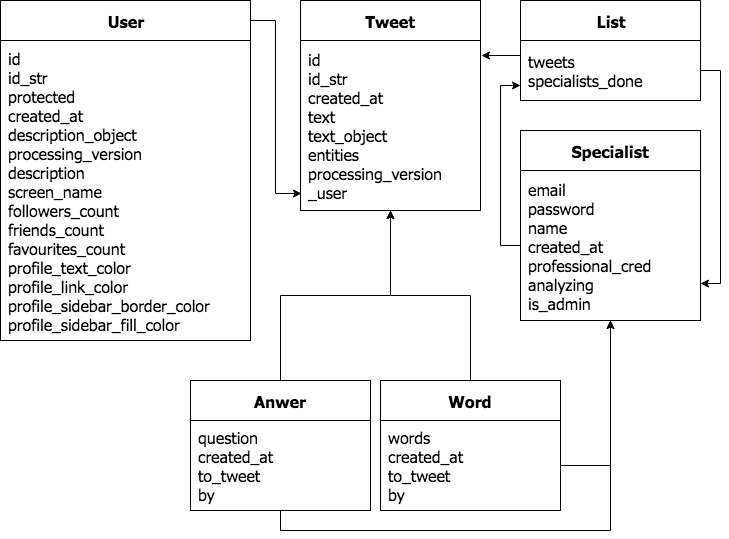
\includegraphics[width=.8\textwidth]{imagens/entities.png}
    \caption{Mapa de entidades do projeto}
    \label{fig:entities}
\end{figure}

Como dito anteriormente, o Docker ja foi préviamente configurado, e assim que você rodar qualquer um dos serviços o mongo local ja estara pronto para receber dados. Entretando, se existir a intenção de subir a pesquisa publicamente, no anexo pode-se encontrar um pequeno adendo de como configurar um mongo gratuito utilizando a plataforma Atlas. Outra ferramenta relevante é o Robo3T\footnote{\url{https://robomongo.org/download}} uma interface gráfica para explorar seu banco, você pode baixa-la caso queira olhar os dados antes dele ser condensado em um dataset menor.

Para que o coletor funcione e insira dados no mongo é necessário configurar as apis do Twitter e a do Google Language.